
\section{Il comportamento degli utenti}

	Nel 1990 e 1991 si sono effettuati diversi sudi sul comportamento degli utenti con metodologie varie. Da questi è sorto che per ogni tipo di media l'uomo mette in atto delle regole ben precise. 
	Vedremo un esempio di media classico e il perché le sue regole \textbf{non} sono da riutilizzare nel web, quali sono le differenze e quali strumenti abbiamo a disposizione per diminuire gli sforzi dell'utenza.
	
	\subsection{Un media classico: Il giornale}
	
		Nel giornale la principale fonte di attrazione è costituita dalle immagini, dalle foto. Più colorate sono più per lo \emph{scanning} quel blocco è fonte di informazione.
		
		\subsubsection{L'importanza delle immagini}
		
			Sui giornali le immagini vincono sul testo 80 a 20. I pezzi di testo accompagnati da immagini infatti risultano quelli più letti. \textbf{L'immagine più grande} è il primo \textbf{punto d'entrata} e d'attrazione primaria per invogliare l'utente alla lettura. Inoltre in un giornale due pagine aperte sono percepite come un'unica grande pagina.
		
	\subsection{Il web}
	
		Alla luce di queste informazioni del comportamento tenuto dagli utenti con i giornali si può forse pernsare che per le pagine web sia lo stesso. Non è così! La modalità di lettura differisci ma non solo, anche lo spostamento dell'attenzione ha un comportamento diverso.
		
		\subsubsection{Fasce d'attenzione}
		
			Per misurare il movimento fatto da utenti in una pagina web si usa la tecnica dell'\emph{eyetracking} da cui si ricava una termografia di una pagina dove le zone calde corrispondono alle dove l'utente dedica più tempo mentre quelle più fredde quelle che non vede affatto se non nella prima fase di \emph{scanning}. Le diverse termografie classiche indicano che il \textbf{punto d'entrata} di una pagina web è \textbf{in alto a sinistra}. Le fasce d'attenzione risultano quindi avere una forma a \emph{F} o a \emph{cono gelato} come si può notare nella figura ~\ref{fig:FasceDAttenzione}.
			Nella maggioranza dei casi per ogni schermata della stessa pagina abbiamo una forma a \emph{F} nel punto in cui avviene lo \emph{scroll} si ha il \emph{blind spot} un punto cieco che non sarà mai visualizzato.
			
			\begin{figure}
				\centering
				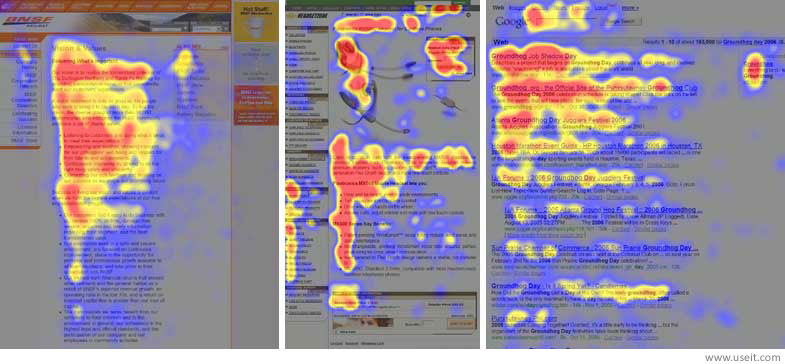
\includegraphics[trim={0 1pt 0 0}, width=\textwidth]{images/IlComportamentoDegliUtenti-FasceDAttenzione}
				\caption[Il comportamento degli utenti - Termografie]{Il comportamento degli utenti - Esempi di termografie}
				\label{fig:FasceDAttenzione}
			\end{figure}
		
		\subsubsection{L'importanza del testo}
			Al contrario dei giornali il testo è molto più rilevante rispetto alle immagini nel web. Per sfruttare questo ecco alcuni consigli per migliorare una pagina web.
			\begin{itemize}
				\item Il punto d'attrazione (in alto a sinistra) necessita di testo, il logo deve essere sempre accompagnato da qualche scritta magari che risponda all'asse What.
				\item Il testo su una singola colonna è meglio che su più colonne come nei giornali (l'effetto è molto simile alle liste \emph{itemize} orizzontali).
				\item Le \emph{keyword} messe vicine diluiscono l'importanza data nello \emph{scan}.
				\item Il \emph{bold} non basta per evidenziare le parole chiave. Meglio usare anche la sottolineatura (come un hyperlink) e ingrandire il \emph{font} o meglio ancora separare la o le \emph{keyword} in una riga a parte (una sorta di mini titolo).
			\end{itemize}
		
			\paragraph{Paragrafi e titoli}
				Un altro utile accorgimento per sfruttare l'importanza del testo è quello di dividere i grandi blocchi di testo in paragrafi corti (rispetto a quelli lunghi attraggono alla lettura quasi il doppio). Lo stesso possiamo dire dei titoli, più sono corti meglio è. Inoltre più un testo è spezzato in piccoli paragrafi più gli utenti sono incoraggiati a leggerlo rilassando i timer (suggerimento valido anche nelle mail).
				Sfruttare il \emph{blurp}, cioè aggiungere ad ogni titolo una mini descrizione per migliorare l'attrazione dell'intera pagina. I \emph{blurp} offrono vantaggi:
				\begin{itemize}
					\item rilassano i timer, ma non cambiano la voglia di proseguire nella navigazione del sito;
					\item aumentano il tasso di ritorno della pagina.
				\end{itemize}
				Il contenuto del \emph{blurp} non è un blocco unico ma può essere suddiviso in parti per cui ha una sua struttura e una sua termografia, per questo motivo le parole fondamentali devono stare alla sinistra del \emph{blurp}.
			
		\subsubsection{Pagine grasse o magre?}
			Per pagina grassa si intende una pagina web con contenuto più spaziato mentre con la pagina snella una pagina con contenuto più compatto. Dalle analisi è emerso che la pagina grassa funziona peggio. Bisogna infatti porre molta attenzione al separare il testo in paragrafi perché si può incorrere nel \emph{diluited design}. La spaziatura e la separazione portano ad uno \emph{scanning} più veloce ma ciò funziona male nelle pagine ricche di contenuto testuale. In generale:
			\begin{itemize}
				\item la \textbf{pagina grassa} è da preferire in quelle pagine di navigazione con link e poco \emph{scroll};
				\item la \textbf{pagina magra} invece è da preferire in quelle pagine con molto contenuto e tanto \emph{scroll}.
			\end{itemize}
		
		\subsubsection{Immagini nel web}
			Abbiamo visto che le immagini nel web hanno un ruolo marginale rispetto al testo difatti un'immagine affiancata ad un testo perde quasi tutta l'attenzione. Nonostante questo hanno comunque una proprietà (diversa dal testo) che le rende utili se sfruttata al meglio. Innanzitutto fissiamo una taglia minimi: 210x230 pixel, più piccola sembra un'icona e c'è rischio di ingannare l'utente. Le immagini hanno un tasso di click superiore al testo, solitamente il 20\% degli utenti clicca sull'immagine. Per sfruttare questo tutte le immagini dovrebbero essere cliccabili con evento correlato, l'utente è abituato cliccarci sopra e si aspetta sempre qualcosa.
			
			\paragraph{Slideshow}
			
		\subsubsection{Lo spostamento dell'utente}
		
			
		
			\paragraph{Legge di Fitts}
			
				\subparagraph{Past\&clink o drag\&drop?}
			
				\subparagraph{Implicazioni della legge di Fitts}
				\subparagraph{Complicazioni}
				
				\subparagraph{Bordi e angoli}
				
				\subparagraph{Menu 2.0}
				
				